%%%%%%%%%%%%%%%%%%%%%%%%%%%%%%%%%%%%%%%%%
% FRI Data Science_report LaTeX Template
% Version 1.0 (28/1/2020)
% 
% Jure Demšar (jure.demsar@fri.uni-lj.si)
%
% Based on MicromouseSymp article template by:
% Mathias Legrand (legrand.mathias@gmail.com) 
% With extensive modifications by:
% Antonio Valente (antonio.luis.valente@gmail.com)
%
% License:
% CC BY-NC-SA 3.0 (http://creativecommons.org/licenses/by-nc-sa/3.0/)
%
%%%%%%%%%%%%%%%%%%%%%%%%%%%%%%%%%%%%%%%%%


%----------------------------------------------------------------------------------------
%	PACKAGES AND OTHER DOCUMENT CONFIGURATIONS
%----------------------------------------------------------------------------------------
\documentclass[fleqn,moreauthors,10pt]{ds_report}
\usepackage[english]{babel}

\graphicspath{{fig/}}




%----------------------------------------------------------------------------------------
%	ARTICLE INFORMATION
%----------------------------------------------------------------------------------------

% Header
\JournalInfo{FRI Natural language processing course 2025}

% Interim or final report
\Archive{Project report} 
%\Archive{Final report} 

% Article title
\PaperTitle{Automatic generation of Slovenian traffic news for RTV Slovenija} 

% Authors (student competitors) and their info
\Authors{Vid Kobal, Matija Tomažič, and Žan Luka Nusdorfer}

% Advisors
\affiliation{\textit{Advisors: Slavko Žitnik}}

% Keywords
\Keywords{prompt engineering, text generation, traffic news, fine-tuning, data-to-text generation, RTV Slovenija}
\newcommand{\keywordname}{Keywords}


%----------------------------------------------------------------------------------------
%	ABSTRACT
%----------------------------------------------------------------------------------------

\Abstract{
This project investigates the use of large language models (LLMs) for automatic generation of Slovenian traffic news reports based on structured data from the promet.si portal. The goal is to replace the current manual workflow at RTV Slovenija with a scalable, automated solution suitable for radio broadcast. Due to infrastructure limitations, we focus on prompt engineering rather than fine-tuning. We experiment with several prompting strategies — zero-shot, few-shot, chain-of-thought, and their combinations — and evaluate the results using both automatic metrics (BLEU, BERTScore) and human judgment. To improve alignment between structured inputs and natural language reports, we develop a preprocessing pipeline that includes HTML cleaning, time-based grouping, and semantic matching using TF-IDF and BERT embeddings. Our findings show that prompt quality alone is not sufficient: the combination of well-prepared data and structured prompting (especially CoT + few-shot) yields the most accurate and editorially consistent outputs. This demonstrates the viability of prompt-based approaches for data-to-text generation in low-resource, domain-specific applications.
}

%----------------------------------------------------------------------------------------

\begin{document}

% Makes all text pages the same height
\flushbottom 

% Print the title and abstract box
\maketitle 

% Removes page numbering from the first page
\thispagestyle{empty} 

%----------------------------------------------------------------------------------------
%	ARTICLE CONTENTS
%----------------------------------------------------------------------------------------

\section*{Introduction}
In an effort to modernize and automate the generation of traffic news for RTV Slovenija, this project explores the application of natural language processing (NLP) techniques for the automatic generation of Slovenian traffic reports. The aim is to create a system that produces short, relevant and stylistically appropriate traffic reports using structured data from the promet.si portal. These reports are intended for radio presenters who regularly read them to inform the public.\newline

The task is currently being done manually. While functional, this approach is more labor-intensive, prone to variability, and limited in terms of scalability. By automating the process, we hope to improve efficiency, consistency, and content quality, while following the editorial standards for language style, relevance, and format.\newline

One of the things we focus on is the correct identification of relevant traffic events, accurate road naming, and appropriate text length and filtering. Although we originally planned to fine-tune a language model using methods such as Low-Rank Adaptation (LoRA), technical issues prevented us from running training on the available infrastructure. Instead, we focused on developing and evaluating a variety of prompt engineering strategies (zero-shot, few-shot, chain-of-thought, and their combinations) for generating quality traffic news. We evaluate generated text using automatic (precision, recall, F1) as well as human evaluation metrics.\newline

Overall, the project demonstrates that with careful prompt design and data preparation, LLMs can be effectively used for structured data-to-text generation in real-world, language-specific use cases such as traffic news.


\section*{Related work}
Generating informative traffic news from structured data falls within the broader domain of data-to-text (D2T) generation, specifically under table-to-text generation. The objective is to transform the data entries into concise and reliable reports that are ready for radio broadcasters to read.\newline

Recent research has demonstrated that LLMs, when combined with data cleaning and model fine-tuning, are highly effective for table-to-text generation. For example, the HeLM (Highlighted Evidence augmented Language Model) framework \cite{bian2024helmhighlightedevidenceaugmented} proposes a two-step approach, where a highlighter selects more important rows. The highlighter is then followed by a summarizer that produces human-readable text. This method achieved state-of-the-art BLUE (bilingual evaluation understudy) and ROGUE (Recall-Oriented Understudy for Gisting Evaluation) scores, confirming that pre-selecting important data improves both model performance and text understandability.\newline

While some approaches rely on model fine-tuning to achieve high-quality outputs, our work focuses on a complementary strategy — prompt engineering. Prompt engineering techniques such as zero-shot and few-shot prompting, chain-of-thought reasoning, and self-consistency decoding have proven effective in controlling LLM output without requiring additional training \cite{vatsal2024surveypromptengineeringmethods}. These strategies help guide the model toward relevant and accurate text generation, which is especially valuable in constrained environments or low-resource languages like Slovenian. In traffic news generation, these strategies help guide the model, while also helping it avoid unnecessary or irrelevant information.\newline

Practical guidance for prompt engineering is provided by Prompting Guide AI (\url{https://www.promptingguide.ai/}), which offers extensive explanations and specific advice on different prompt engineering approaches. In addition, Ollama has demonstrated effective prompt workflow with models like Code Llama, especially for tasks involving structure data transformation. They offer different examples on how to prompt Code Llama to optimize relevance and clarity (\url{https://ollama.com/blog/how-to-prompt-code-llama}).\newline

Although parameter-efficient fine-tuning methods like LoRA \cite{lowrandadaptation} and QLoRA \cite{qlora} are promising for domain-specific adaptation on limited hardware, we did not pursue this direction due to infrastructure issues. However, existing research confirms that prompt engineering can serve as a strong alternative, especially when combined with high-quality data preprocessing.

\section*{Data \& Preprocessing}

The input data for this project was obtained from the promet.si portal in CSV format. Each entry corresponds to a traffic report, containing multiple fields such as road names, event categories, timestamps, etc. The raw data included HTML tags and several fields that were irrelevant or redundant for the purpose of generating public traffic reports. These included metadata such as operator names, and frequently repeating elements like generic holiday restrictions for freight vehicles, which were often not relevant. As a first step, we removed HTML tags, stripped boilerplate text, and filtered out irrelevant sections.\newline

Since the final traffic reports are read on air in predefined intervals, we grouped the structured entries from the CSV into meaningful time segments to simulate these reporting periods. Duplicate entries and near-duplicates were merged or removed to avoid redundancy.\newline

To create training pairs, we used a collection of RTF files containing previously written traffic reports. Our initial approach attempted to align grouped CSV entries with RTF reports using timestamp matching with a time tolerance window. However, this method proved unreliable due to timing mismatches and inconsistencies. Instead, we calculated TF-IDF similarity scores between structured inputs and RTF outputs, and if the score exceeded a chosen threshold, we linked them as input-output pairs; to ensure sufficient data for evaluation, we applied a slightly lower threshold, which led to some imperfect matches and consequently affected the performance of automatic metrics.

\section*{Methods}
To improve the quality of our traffic reports, we will leverage various prompt engineering techniques such as few-shot prompting, which provides examples to guide the model’s responses; chain-of-thought prompting, which encourages step-by-step reasoning for better accuracy; and prompt chaining, where multiple prompts are linked together to refine and build upon previous outputs.
These techniques help ensure more accurate, detailed, and contextually relevant traffic reports.

\subsection*{Zero-shot prompting}
Zero-shot prompting is a technique where we provide the model with a task description and ask it to generate a response without any examples.
This strategy relies on the model being adequately trained and being exposed to large amounts of data, which allows it to generalize and understand the task at hand.

\subsection*{Few-shot prompting}
Few-shot prompting involves providing the model with a few examples of the desired input-output format before asking it to generate a response.
It helps the model understand the pattern of the expected output.

\subsection*{Chain-of-thought prompting (CoT)}
Chain-of-thought prompting is a technique that encourages the model to break down its reasoning process step by step, by asking the model to explain its thought process.

\subsection*{Prompt chaining}
Prompt chaining is a technique where we link multiple prompts together to refine and build upon the model's previous outputs.
This approach allows us to create a more structured and coherent response by guiding the model through a series of related tasks or questions.

\subsection*{Self-consistency prompting} Self-consistency prompting involves generating multiple outputs for the same prompt and selecting the most appropriate one. This helps reduce variability in model responses and improves reliability. It is especially useful with models like GaMS 9B, which may produce inconsistent results across runs.

\subsection*{Implementation}
In the early phase of the project, we evaluated several prompting strategies using the GaMS-9B-Instruct language model. However, the input data at that stage was not yet fully cleaned: HTML tags remained, and data alignment relied only on timestamps without verifying content similarity. This led to inconsistent and often inaccurate outputs.\newline

To address these issues, we overhauled the data preprocessing and alignment pipeline. We developed scripts to clean HTML content, group input rows by time, and align structured data with RTF reports more accurately using extracted timestamps and semantic similarity. A key component was test\_distance.py, which used TF-IDF cosine similarity within a sliding time window to match inputs with the most relevant RTF outputs. We later fed the cleaned input into prompt\_generator.py, which handles prompt construction, model invocation, and result storage.\newline

As a result, we achieved more consistent and interpretable outputs. Using TF-IDF (and optionally BERT) similarity scoring, we automatically aligned over 100 useful input-output pairs (similarity greater than 0.6), which supported both evaluation and prompt refinement.

\section*{Results}
Due to technical issues encountered while running our code on the HPC system, we were only able to generate a smaller sample of results than originally planned. Ultimately, we successfully produced 232 traffic reports using the GaMS-9B model. These reports were generated using four different prompting techniques: zero-shot, few-shot, chain-of-thought (CoT), and a combination of CoT and few-shot.\newline

In the early phase of the project, we manually evaluated a smaller sample of outputs, generated using uncleaned data and loosely aligned input-output pairs. In this preliminary setup, the best-performing strategy was CoT combined with few-shot prompting, followed by few-shot alone, then chain-of-thought, and finally zero-shot prompting.\newline

After improving the data cleaning and alignment process, and re-running the full evaluation pipeline using \newline {prompt\_generator.py}, the results shifted, highlighting the importance of high-quality input-output pairs for both prompting performance and metric reliability.

\begin{figure}[h!]
  \centering
  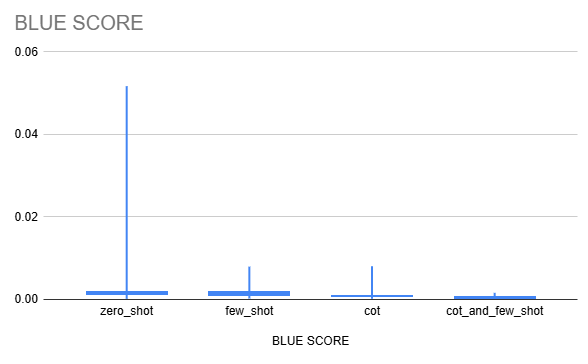
\includegraphics[scale=0.4]{fig/blue_score.png}
  \caption{Prompting techniques BLUE score results.}
  \label{fig:blue}
\end{figure}
\begin{figure}[h!]
  \centering
  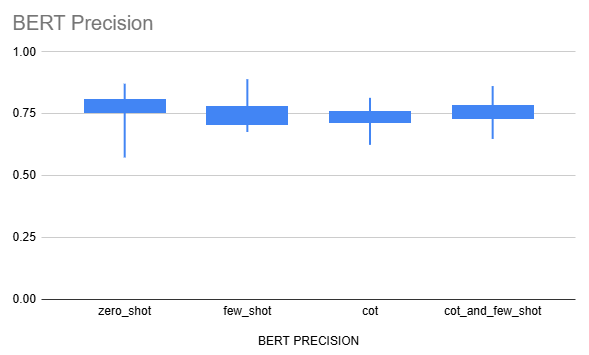
\includegraphics[scale=0.4]{fig/bert_precision.png}
  \caption{Prompting techniques BERT precision score results.}
  \label{fig:bert_pre}
\end{figure}
\begin{figure}[h!]
  \centering
  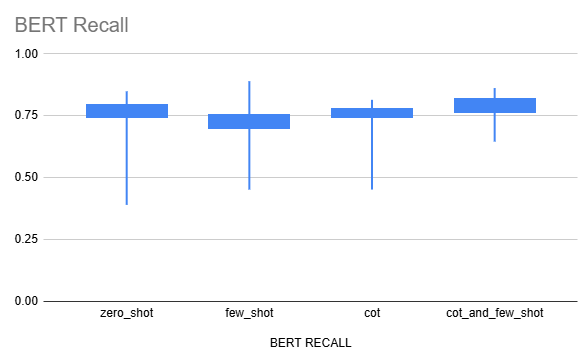
\includegraphics[scale=0.4]{fig/bert_recall.png}
  \caption{Prompting techniques BERT recall score results.}
  \label{fig:bert_recall}
\end{figure}
\newpage
\begin{figure}[h!]
  \centering
  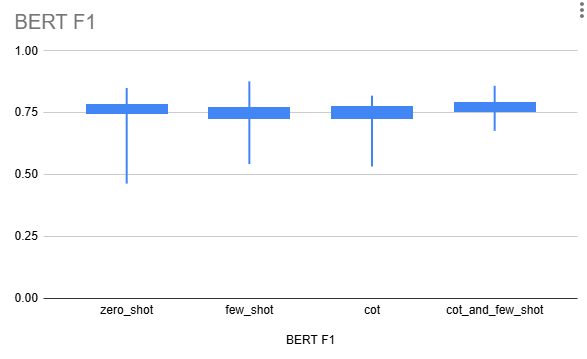
\includegraphics[scale=0.4]{fig/bert_f1.png}
  \caption{Prompting techniques BERT F1 score results.}
  \label{fig:bert_f1}
\end{figure}

\subsection*{Automatic evaluation}

To evaluate the performance of the generated traffic reports, we used a combination of automatic and human evaluation methods. For automatic evaluation, we integrated the computation of two key metrics directly into the \newline prompt\_generator.py pipeline:

\begin{itemize}
    \item BLEU (Bilingual Evaluation Understudy, see figure \ref{fig:blue}), which compares the overlap of n-grams between the generated and reference texts.
    \item BERTScore (see figures \ref{fig:bert_pre}, \ref{fig:bert_recall}, \ref{fig:bert_f1}), which uses contextual embeddings from BERT to evaluate semantic similarity between outputs and references.
\end{itemize}

The evaluation of prompting techniques revealed that the combination of chain-of-thought (CoT) and few-shot prompting achieved the best overall performance, with the highest BERT F1 score. This indicates that combining structured reasoning with example-based guidance leads to more accurate outputs.\newline

Surprisingly, zero-shot prompting performed nearly as well, even outperforming both few-shot and CoT when used individually. This challenges the common assumption that more elaborate prompting strategies are always more effective.\newline

When applied separately, few-shot and CoT prompting showed weaker results, suggesting that neither examples nor reasoning alone were sufficient. Their combination, however, proved significantly more effective.\newline

Compared to our initial experiments — which used uncleaned and poorly aligned data — zero-shot prompting now performed much better, closing the gap with more advanced techniques. This highlights that, in the context of prompt engineering, input data quality and preprocessing can have an equal or even greater impact on final performance than the choice of prompting strategy itself.\newline

In addition, due to the specific nature of the task (radio-ready structured text in Slovenian), we also conducted human evaluation on a selected subset of generated reports. Each report was assessed across several qualitative dimensions; fluency, grammatical correctness, format and structure, naming accuracy, information ordering, factual consistency, relevance and brevity.\newline

\subsection*{Manual evaluation}
Our qualitative, manual evaluation of all tested prompting strategies revealed that all techniques produce generally fluent and grammatically correct outputs. Across all variants, average scores for fluency and grammar were consistently high, with only minor stylistic or syntactic issues. These issues could likely be mitigated by using a larger model such as GAMS 27B, provided sufficient compute resources.\newline

Format adherence, however, varied significantly across techniques. The weakest formatting was observed in zero-shot and few-shot outputs, which frequently omitted structural elements of the report. Chain-of-thought outputs improved slightly in this respect but remained inconsistent. As expected, the CoT + few-shot technique performed best, as it combined clear instructions with concrete examples.\newline

Across all evaluation categories — naming conventions, information ordering, factual consistency, and overall relevance — the combination of chain-of-thought and few-shot prompting consistently outperformed other methods. This approach led to more precise road naming, better prioritization of major incidents, higher factual accuracy, and more relevant content. CoT alone typically ranked second, offering reasonable structure and coverage, while zero-shot prompting achieved surprisingly competitive results despite its simplicity. Few-shot prompting, on the other hand, often underperformed by producing overly brief outputs that omitted critical details — an unexpected result, considering that the model was provided with additional guidance through examples. These trends reinforce the value of combining structured reasoning with concrete examples and highlight the limitations of relying on either technique in isolation.

\section*{Discussion}

Our results show that prompt engineering, when supported by robust data preprocessing, is an effective approach for structured data-to-text generation in Slovenian traffic reporting. Initial outputs were weak due to uncleaned data and imprecise alignment, but improvements such as HTML stripping, time-based grouping, and semantic similarity matching (TF-IDF/BERT) led to significantly more accurate and consistent results.\newline

Among tested strategies, the combination of chain-of-thought and few-shot prompting yielded the best performance across both automatic (BERT F1) and human evaluation metrics. This confirms that structured reasoning combined with examples helps models better follow both the content and editorial conventions of traffic reports.\newline

Surprisingly, zero-shot prompting performed better than expected after cleaning, sometimes even outperforming few-shot and CoT alone. This highlights that preprocessing quality can play an equally — or more — important role than prompt complexity itself.\newline

Few-shot prompting alone often underperformed due to brief, incomplete outputs, likely caused by token limitations or suboptimal example phrasing. These observations underscore that prompt effectiveness depends not only on the technique but also on prompt design and input structure.\newline

Despite these advances, limitations remain. Prompt outputs are still variable and sensitive to small changes; semantic matching may not fully capture context; and infrastructure constraints prevented comparisons with fine-tuned models. Additionally, some outputs contained minor inaccuracies, suggesting that hybrid systems — combining LLMs with rule-based filters — could improve factual consistency.

\section*{Conclusion}

This project explored the use of large language models for automatic generation of Slovenian traffic news, based on structured data from the promet.si portal. Despite initial limitations due to uncleaned data and simple timestamp matching, we successfully built a comprehensive preprocessing and prompting pipeline that significantly improved output quality. By leveraging prompt engineering techniques and semantic similarity for data alignment, we generated fluent, relevant, and stylistically appropriate reports. While we were not successfull at fine-tuning, our results show that carefully designed prompt-based methods, combined with human and automatic evaluation, can offer a robust solution for domain-specific text generation tasks — even in low-resource languages like Slovenian.


\bibliographystyle{unsrt}
\bibliography{report}

\end{document}